% !TEX TS-program = pdflatex
% !TEX encoding = UTF-8 Unicode

% This is a simple template for a LaTeX document using the "article" class.
% See "book", "report", "letter" for other types of document.

\documentclass[11pt]{article} % use larger type; default would be 10pt

\usepackage[utf8]{inputenc} % set input encoding (not needed with XeLaTeX)

%%% Examples of Article customizations
% These packages are optional, depending whether you want the features they provide.
% See the LaTeX Companion or other references for full information.

%%% PAGE DIMENSIONS
\usepackage{geometry} % to change the page dimensions
\geometry{a4paper} % or letterpaper (US) or a5paper or....
% \geometry{margin=2in} % for example, change the margins to 2 inches all round
% \geometry{landscape} % set up the page for landscape
%   read geometry.pdf for detailed page layout information

\usepackage{graphicx} % support the \includegraphics command and options
\usepackage{alltt}
\usepackage{wrapfig}
% \usepackage[parfill]{parskip} % Activate to begin paragraphs with an empty line rather than an indent

%%% PACKAGES
\usepackage{booktabs} % for much better looking tables
\usepackage{array} % for better arrays (eg matrices) in maths
\usepackage{amssymb}
\usepackage{paralist} % very flexible & customisable lists (eg. enumerate/itemize, etc.)
\usepackage{verbatim} % adds environment for commenting out blocks of text & for better verbatim
\usepackage{subfig} % make it possible to include more than one captioned figure/table in a single float
% These packages are all incorporated in the memoir class to one degree or another...

%%% HEADERS & FOOTERS
\usepackage{fancyhdr} % This should be set AFTER setting up the page geometry
\pagestyle{fancy} % options: empty , plain , fancy
\renewcommand{\headrulewidth}{0pt} % customise the layout...
\lhead{}\chead{}\rhead{}
\lfoot{}\cfoot{\thepage}\rfoot{}

%%% SECTION TITLE APPEARANCE
\usepackage{sectsty}
\allsectionsfont{\sffamily\mdseries\upshape} % (See the fntguide.pdf for font help)
% (This matches ConTeXt defaults)

%%% ToC (table of contents) APPEARANCE
\usepackage[nottoc,notlof,notlot]{tocbibind} % Put the bibliography in the ToC
\usepackage[titles,subfigure]{tocloft} % Alter the style of the Table of Contents
\renewcommand{\cftsecfont}{\rmfamily\mdseries\upshape}
\renewcommand{\cftsecpagefont}{\rmfamily\mdseries\upshape} % No bold!

%%% END Article customizations

%%% The "real" document content comes below...

\title{Numerical Analysis Project 3}
\author{Margaret Dorsey}
%\date{} % Activate to display a given date or no date (if empty),
         % otherwise the current date is printed 

\newenvironment{claim}[1]{\par\noindent\underline{Claim:}\space#1}{}
\newenvironment{proof}[1]{\par\noindent\underline{Proof:}\space#1}{\hfill $\blacksquare$}

\newcommand{\pder}[2][]{\frac{\partial#1}{\partial#2}}

\begin{document}
\maketitle

\section*{Background}
\subsection*{$n = .5$}

$\Xi = $
$-\left(\pder[\theta]{\xi}\right)_{\xi = \Xi} = $

\begin{tabular}{| c | c c c c c |}
\hline
$\xi$ & $\theta$ & $\hat{M}$ &  $\hat{I}$  & $\hat{\Omega}$ \\
\hline

\hline
\end{tabular}

\subsection*{$n = 1$}


\subsection*{$n = 2$}


\subsection*{$n = 3$}

%\begin{tabular}{| c | c c c c c |}
%\hline
%n & $\hat{M}$ & $\Xi$ & $-\left(\pder[\theta]{\xi}\right)_{\xi = \Xi}$ & $\hat{\Omega}$ & $\hat{I}$ \\
%\hline
%0.5 & & & & & \\
%1.0 & & & & & \\
%2.0 & & & & & \\
%3.0 & & & & & \\
%\hline
%\end{tabular}

\subsection*{Modelling Earth's Sun}

\section{White Dwarfs}
\subsection*{$\pder[V]{s}$}
\subsection*{Integrations for Selected Values of $\theta(0)$}
%\begin{figure}
%\begin{tabular}{c c}
 % 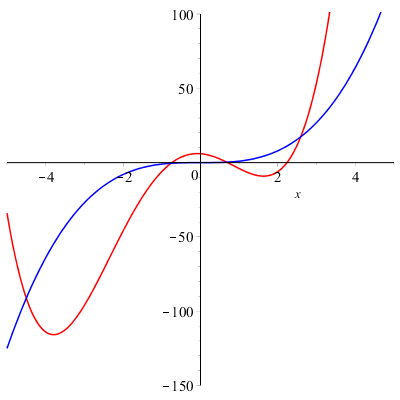
\includegraphics[width=0.5\textwidth]{problem1plot2.png} &   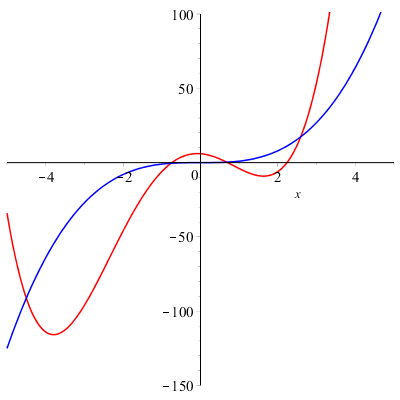
\includegraphics[width=0.5\textwidth]{problem1plot2.png} \\
%$\theta(0) = $ & $\theta(0) = $ \\[6pt]
%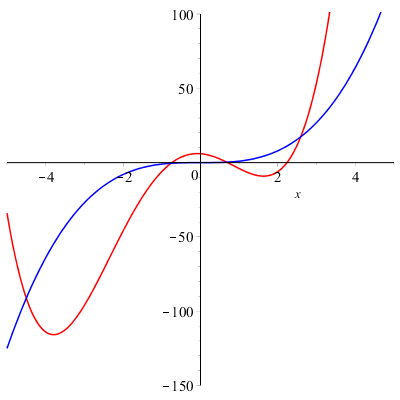
\includegraphics[width=0.5\textwidth]{problem1plot2.png} &   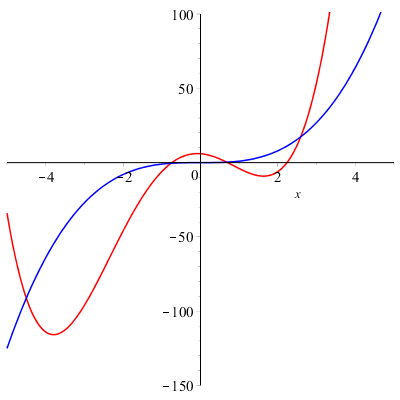
\includegraphics[width=0.5\textwidth]{problem1plot2.png} \\
%$\theta(0) = $ & $\theta(0) = $ \\[6pt]
% 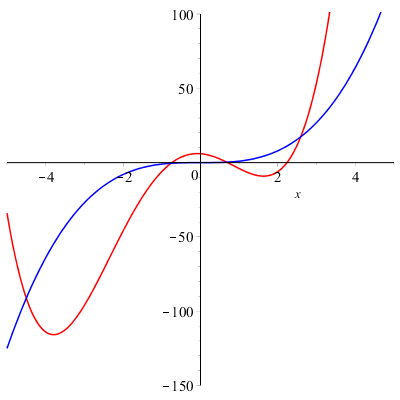
\includegraphics[width=0.5\textwidth]{problem1plot2.png} &   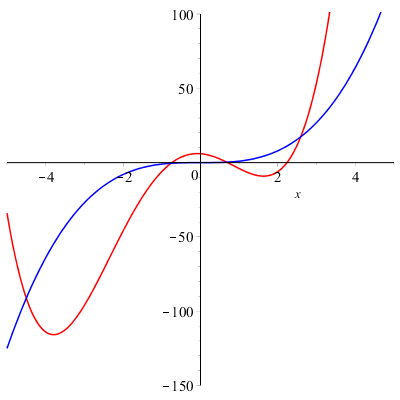
\includegraphics[width=0.5\textwidth]{problem1plot2.png}\\
%$\theta(0) = $ & $\theta(0) = $ \\[6pt]
% 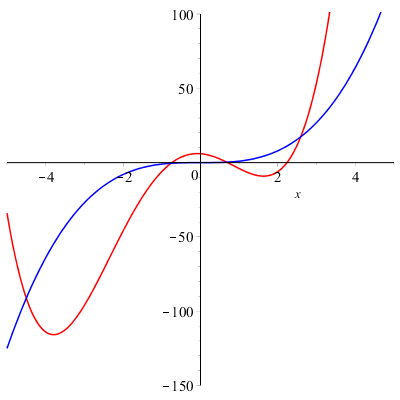
\includegraphics[width=0.5\textwidth]{problem1plot2.png} &  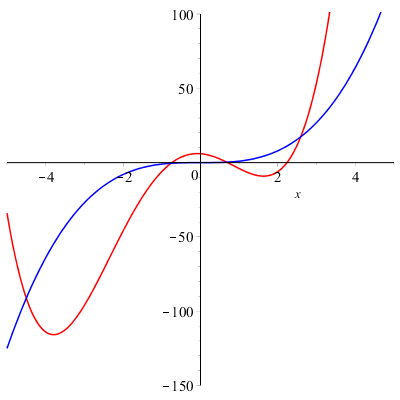
\includegraphics[width=0.5\textwidth]{problem1plot2.png} \\
%$\theta(0) = $ & $\theta(0) = $ \\[6pt]

%\end{tabular}
%\end{figure}

\subsection*{Dimensionless Mass}

\subsection*{Mass-Radius Relation}




